W tym rozdziale przedstawiono przykłady systemów, narzędzi oraz technik nawigacyjnych, które są wykorzystywane w usługach firm komercyjnych 
oraz w dostarczanych przez te firmy systemach rolnictwa precyzyjnego. Z uwagi na niską dostępność specyfikacji technicznych produktów 
dostępnych obecnie na rynku, w pracy ogranioczono się do analizy ofert marketingowych liderów branży maszyn rolniczych.
Jako reprezentatywną próbę dla europejskiego rynku rolnictwa precyzyjnego przyjęto oferty następujących firm: New Holland Agriculture,
John Deere oraz Claas.
\section{Wykorzystanie GNSS}
% test cytowania \cite{CLAAS_stearing_systems}\\
%	test cytowania \cite{JOHN_DEERE_solutions}\\
%	test cytowania \cite{NEW_HOLLAND_PLM}
W tym podrozdziale w formie porównania wykorzystywanych systemów pozycjonowania a także oferowanych technik wyznaczania pozycji opisano wykorzystanie 
systemów GNSS przez firmy komercyjne z grupy wybranej jako reprezentatywna.\\
\indent Na wstępie należy uściślić pojęcia dokładności, które pojawiały się w broszurach marketingowych, a które nie zawsze były rzetelnie opisywane 
przez firmy refereujące o swoich produktach. Z reguły gdy w broszurach podawana jest dokładność, brakuje informacji odnośnie poziomu ufności\footnote{
W przypadku wyznaczania pozycji poziom ufności bezpośrednio określa prawdopodobieństwo zawarcia wartości prawdziwej (prawdziwe położenie) w okręgu o środku w punkcie 
estymowanym i promieniu równym odpowiednio: 1$\sigma$ P=68\%; 2$\sigma$ P=95\%; 3$\sigma$ P=99.7\%, gdzie $\sigma$ oznacza odchylenie standardowe estymowanej pozycji.}
oraz czy jest to dokładność w sensie absolutnym czy może dokładność podawana jest relatywnie w stosunku do kolejnych wyznaczeń tym samym odbiornikiem - tzw.
dokładnośc między-przejazdowa (pass to pass accuracy). Typ uzyskiwanej dokładności - relatywna czy absolutna rzutuje bezpośrednio na rodzaj zabiegów 
agrotechnicznych, które możemy wykonywać. Dla przykładu przy zakładaniu ścieżek przejazdowych, które mają służyć przez cały sezon wegetacyjny potrzebna 
jest wysoka dokładność w sensie absolutnym, natomiast w celu eliminacji omijaków bądź nakładek przy zabiegach agrotechnicznych wystarczy dokładność między-przejazdowa.
Aby uniknąć nieporozumień nacisk połorzono na porównanie wykorzystywanych technologii. Wszędzie tam gdzie w broszurach marketingowych nie wyspecyfikowano typu 
dokładności w pracy zamieszczono oba rodzaje zaczerpnięte z literatury lub strony producenta.\\
\indent Wszystkie trzy firmy oferują w swoim portfolio odbiorniki mające możliwość odbioru sygnału zarówno GPS jak i GLONASS w dwóch częstotliwościach.
Firma John Deere ma w swojej ofercie odbiornik StarFire 3000 rysunek \ref{fig:john_deere_starfire}. Firma Class oferuje Antenę GPS PILOT wraz z terminalem S7
\ref{fig:class_antena} i komputerem nawigacyjnym przedstawionym na rysunku \ref{fig:class_navigation_computer}, natomiast 
firma New Holland Agriculture w swojej ofercie prezentuje kilka rodzajów anten oraz odbiorników w zależności od wymaganej dokładności. Przykładem jest odbiornik 
NH 372 przedstawiony na rysunku \ref{fig:new_holland_nh372}.
\begin{figure}[H]
\centering
        \begin{subfigure}{0.3\textwidth}
                \centering
                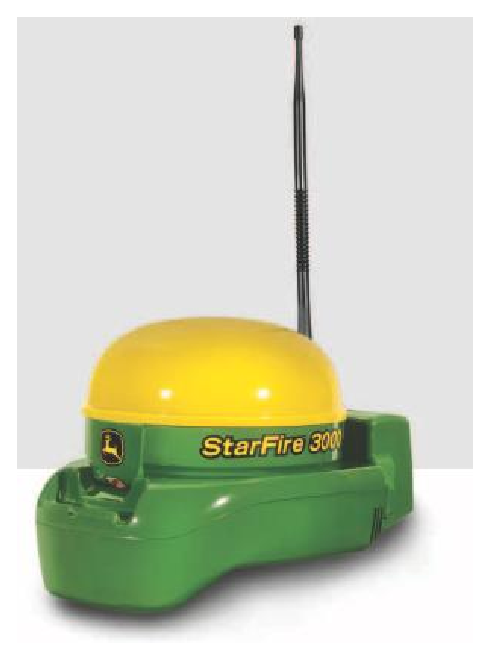
\includegraphics[width=0.9\linewidth]{ch5_john_deere_starfire.eps}
                \caption{Odbiornik StarFire 3000 firmy John Deere}
                \label{fig:john_deere_starfire}
        \end{subfigure}
        %\hfill
        \begin{subfigure}{0.3\textwidth}
                \centering
                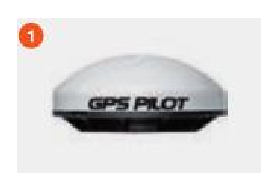
\includegraphics[width=0.9\linewidth]{ch5_class_antena.eps}
                \caption{antena GPS PILOT firmy Class}
                \label{fig:class_antena}
        \end{subfigure}
        \begin{subfigure}{0.3\textwidth}
                \centering
                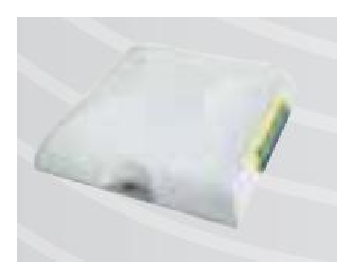
\includegraphics[width=0.9\linewidth]{ch5_new_holland_receiver.eps}
                \caption{odbiornik NH 372 firmy New Holland Agriculture}
                \label{fig:new_holland_nh372}
        \end{subfigure}
\caption{Przegląd komercyjnych odbiorników GNSS}
\end{figure}
%%%%%%%%%%%%%%%%%%%%%%%%%%%%EGNOS%%%%%%%%%%%%%%%%%%%%%%%%%%%%%%%%%%%%%%%%%%
\indent Jeżeli weźmiemy pod uwagę publicznie dostępne systemy augmentacyjne GNSS, to europejski system EGNOS jest wykorzystywany 
przez firmy Class oraz New Holland Agriculture. Ponadto firm New Holland oferuje zbliżony dokładnością do systemu EGNOS sygnał korekcyjny OmniStar VBS rysunek
\ref{fig:omnistar_vbs}. Firma John Deere dostarcza swojego własnego rozwiązania w postaci sygnału 
korekcyjnego SF1. Absolutna dokładność rozwiązania GNSS z sygnałem korekcyjnym EGNOS jest na poziomie trzech metrów (2$\sigma$).
Ponieważ, firmy zalecają używanie GNSS z sygnałem korekcyjnym EGNOS do prowadzenia prac uprawowych, w których powtarzalność przejazdów nie 
ma istotnego znaczenia, zatem w ofercie prezentują dokładność relatywną na poziomie $\pm$30cm. Relatywna dokładność GNSS z sygnałem korekcyjnym SF1 od John Deere 
jest podawana na poziomie $\pm$23cm. System EGNOS transmituje poprawki różnicowe dla częstotliwości L1 sygnału GPS za pomocą łącza satelitarnego. Działanie systemu 
przedstawia poniższy rysunek \ref{fig:class_egnos}.
\begin{figure}[H]
\centering
        \begin{subfigure}{0.4\textwidth}
                \centering
                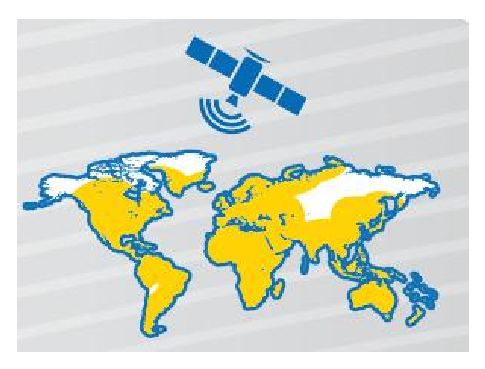
\includegraphics[width=0.9\linewidth]{ch5_new_holland_egnos.eps}
                \caption{\textit{Zasięg sygnału OmniStar VBS} źródło \cite[][strona 4]{NEW_HOLLAND_PLM}}
                \label{fig:omnistar_vbs}
        \end{subfigure}
        \begin{subfigure}{0.4\textwidth}
                \centering
                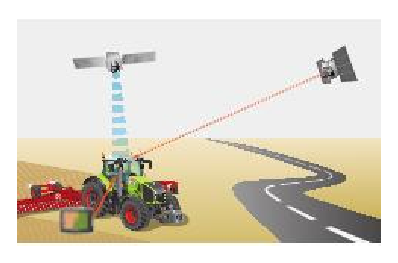
\includegraphics[width=0.9\linewidth]{ch5_class_egnos.eps}
                \caption{\textit{Zasada działania systemu EGNOS według Class} źródło \cite[][strona 26]{CLAAS_stearing_systems}}
                \label{fig:class_egnos}
        \end{subfigure}
\caption{Wykorzystanie sygnału korekcyjnego niskiej jakości}
\end{figure}
\indent 

\section{Zastosowanie systemów inercjalnych}
Na podstawie analizy ofert marketingowych firm z grupy przyjętej za referencyjną, można wywnioskować, że systemy nawigacji inercjalnej 
są wykorzystywane na potrzeby budowy systemów służących do kompensacji nierówności terenu przy precyzyjnym prowadzeniu maszyn rolniczych.
Firma Trimble w swoich technologiach kompensacji terenu T2, T3 wykorzystuje akcelerometry do wyznaczania kąta inklinacji\footnote{kąt zawarty między osią 
pionową pojazu a kierunkiem siły ciężkości w danym punkcie na Ziemi.} oraz żyroskopy w celu kompensacji danych z akcelerometrów ze względu na własną dynamikę pojazdu oraz 
w celu wyznaczania prędkości z jaką zmienia się położenie pojazdu względem kierunku pionu \cite[]{TRIMBLE}.
Z analizowanej grupy firma John Deere oferuje autorskie rozwiązania w postaci modułu kompensacji terenu TCM. Moduł TCM pozwala na wprowadzanie korekt 
do pozycji GNSS ze względu na pochyłości terenu w trzech osiach z, y, z. Moduł kompensacji terenu jest domyślenie zintergrowany z odbiornikiem GNSS StarFire 3000.
Rysunek \ref{fig:john_deere_tcm} przedstawia możliwości systemu TCM. 

\begin{figure}[H]
\centering
\begin{minipage}[c]{0.6\linewidth}
  \begin{flushleft}
  	\begin{minipage}[t]{0.5\linewidth}
		\raggedleft
		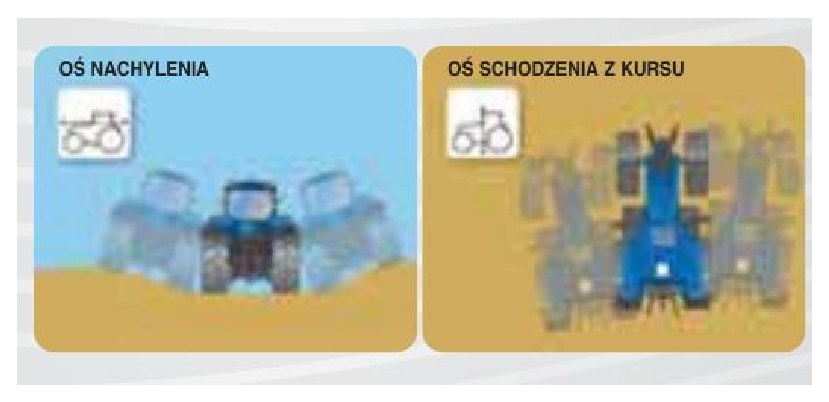
\includegraphics[scale = 0.4]{ch5_new_holland_terrain_compensation_t2.eps}	
		\subcaption{Technologia kompensacji terenu T2 wykorzystywana przez New Holland Agriculture}
		\label{fig:t2}
	\end{minipage}
	\vfill
	\begin{minipage}[b]{0.5\linewidth}
		\raggedleft
		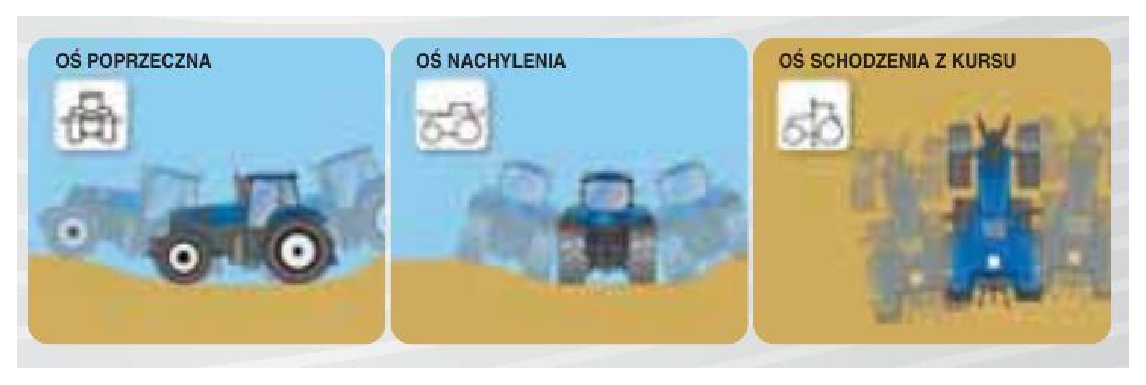
\includegraphics[scale = 0.4]{ch5_new_holland_terrain_compensation_t3.eps}
		\subcaption{Technolohia kompenasacji terenu T3 wykorzystywana przez New Holland Agriculture}
		\label{fig:t3}
	\end{minipage}
  \end{flushleft}
\end{minipage}%
\hfill
\begin{minipage}[c]{0.4\linewidth}
  \begin{flushright}
  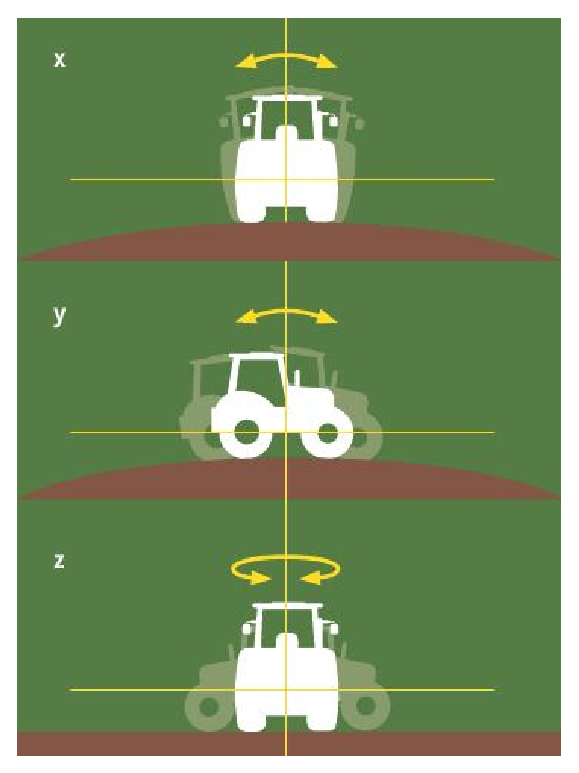
\includegraphics[scale = 0.5]{ch5_john_deere_terrain_compensation.eps}
  \subcaption{\textit{Technologia kompensacji terenu TCM od John Deere} źródło \cite[][strona 8]{JOHN_DEERE_solutions}}
  \label{fig:john_deere_tcm}
  \end{flushright}
\end{minipage}
\caption{\textit{Kompensacja wpływu nierówności terenu na pozycję GNSS}}
\label{fig:terrain_compensation}
\end{figure}
Firma New Holland Agriculture również posiada w swojej ofercie system kompensacji terenu w dwóch różnych wersjach: T2 - z pominięciem kompensacji w 
płaszczyźnie podłużnej, T3 - kompensujący nierówności w obu płasczyznach (poprzeczna, podłużna) oraz zapobiegający schodzeniu maszyny z kursu \cite[][strona 7]{NEW_HOLLAND_PLM}.
Firma New Holland Agriculture najprawdopodobniej wykorzystuje rozwiązania T2 oraz T3 oferowane przez odbiorniki marki Trimble. 
Na rysunku \ref{fig:t2} oraz \ref{fig:t3} przedstawiono schemat działania rozwiązań zaadoptowanych przez New Holland.
Firma Class w swoim portfolio również posiada 6 osiowy żyroskop (żyroskop akcelerometr) do uwzględniania ruchów podłużnych i poprzecznych pojazdu. 
Moduł INS jest wmontowany w specjalny komputer nawigacyjny - rysunek \ref{fig:class_navigation_computer}, 
który wylicza ślady przejazdów oraz wprowadza korekty ze względu na nierówności terenu.\\
\begin{figure}[H]
	\centering
	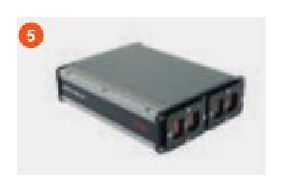
\includegraphics[scale=0.4]{ch5_class_navigation_computer.eps}
	\caption{Komputer do nawigacji Class z wmontowanymi sensorami do kompensacji nierówności terenu}
	\label{fig:class_navigation_computer}
\end{figure}
\indent Warto nadmienić, że firmy obecnie jedynie wykorzystują narzędzia nawigacji inercjalnej (INS) do korekcji rozwiązań GNSS.
Z broszur marketingowych wywnioskować można, że komercyjnie nie stosuje się jeszcze filtru kalmana w celu wspólnego opracowania obserwacji GNSS plus INS.
\section{Zastosowanie sensorów video}
Firma CLASS w swojej ofercie posiada systemy wspomagające nawigację GNSS oparte o sensory wideo. CAM PILOT przedstawiony na rysunku \ref{fig:class_cam_pilot1}
jest systemem automatycznego kierowania sterowanym przez kamerę stereoskopową. Został zaprojektowany specjalnie do zbioru traw. Kamera ustala pozycję pokosów 
i na podstawie tej informacji odbywa się prowadzenie pojazdu \cite[][strona 7]{CLAAS_stearing_systems}.
W ofercie firmy CLASS jest także system oparty na skaningu laserowym LASER PILOT zobrazowany na 
rysunku \ref{fig:class_laser_pilot1} zaprojektowany do ustalania krawędzi między polem skoszonym a jeszcze nie omłuconym. System pozwala na 
prowadzenie pojazdu wzdłuż tej krawędzi z dokładnością 10-20cm \cite[][strona 6]{CLAAS_stearing_systems}.
\begin{figure}[H]
\centering
	\begin{subfigure}{0.4\textwidth}
		\centering
		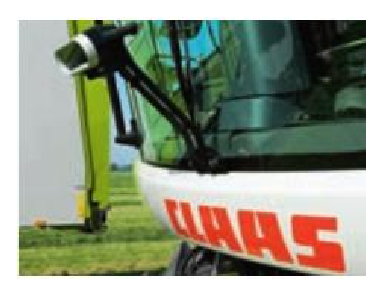
\includegraphics[width=0.9\linewidth]{ch5_class_cam_pilot0.eps}
		\caption{CLASS CAM PILOT}
		\label{fig:class_cam_pilot1}
	\end{subfigure}
	%\hfill
	\begin{subfigure}{0.4\textwidth}
                \centering
                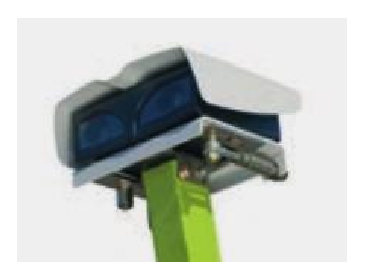
\includegraphics[width=0.9\linewidth]{ch5_class_laser_pilot0.eps}
                \caption{CLASS LASER PILOT}
                \label{fig:class_laser_pilot1}
	\end{subfigure} \\
	\vfill
	\begin{subfigure}{0.4\textwidth}
                \centering
                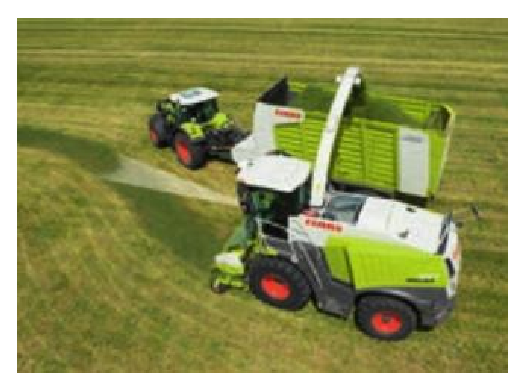
\includegraphics[width=0.9\linewidth]{ch5_class_cam_pilot.eps}
                \caption{CLASS CAM PILOT podczas pracy}
                \label{fig:class_cam_pilot2}
	\end{subfigure}
	\begin{subfigure}{0.4\textwidth}
                \centering
                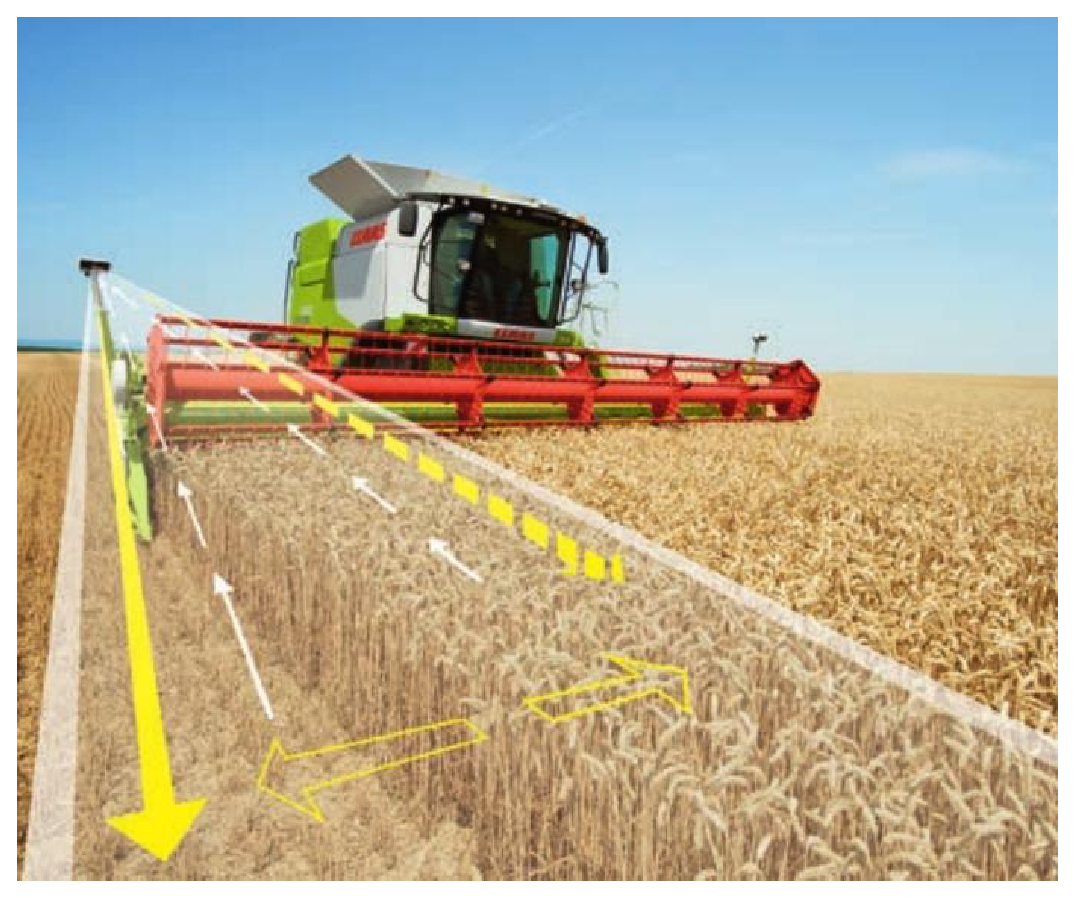
\includegraphics[width=0.9\linewidth]{ch5_class_laser_pilot.eps}
                \caption{CLASS LASER PILOT podczas pracy}
                \label{fig:class_laser_pilot2}
	\end{subfigure}
\caption{Systemy bazujące na sensorach wideo marki CLASS}
\end{figure}
\indent Również firma New Holland Agriculture posiada w swej ofercie system oparty na sensorach wideo.
System SMARTSTEER przedstawiony na rysunku \ref{fig:new_holland_smartsteer} za pomocą skanera laserowego wytycza krawędź dzielącą ściernisko 
od zborza i na podstawie tej informacji przesyła sygnały do układu kierowniczego \cite[][strona 18]{NEW_HOLLAND_PLM}.
\begin{figure}[H]
	\centering
	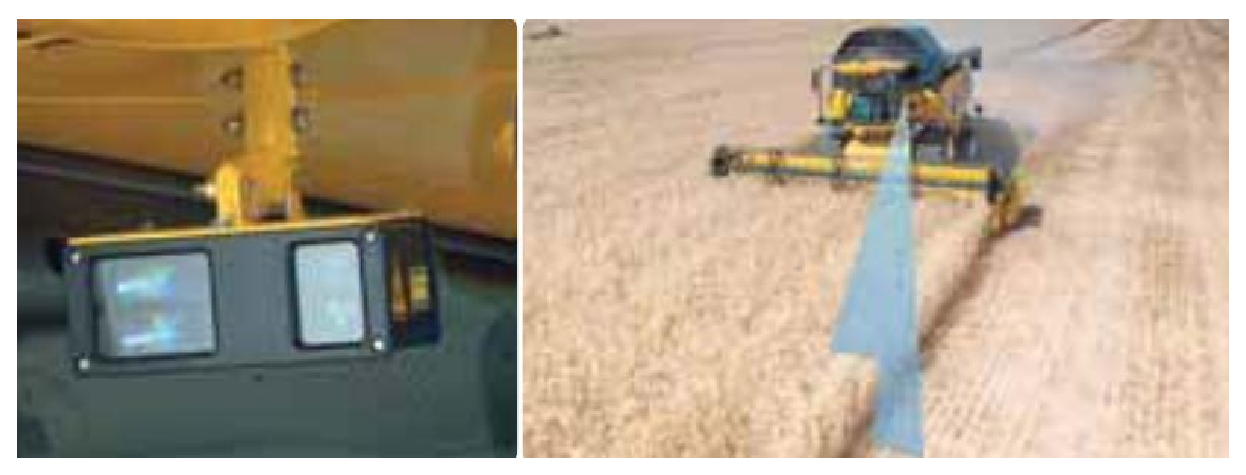
\includegraphics[width=0.7\linewidth]{ch5_new_holland_laser_pilot.eps}
	\caption{System SMARTSTEER firmy New Holland Agriculture}
	\label{fig:new_holland_smartsteer}
\end{figure}
\indent Firma John Deere jako jedyna firma z trzech wybranych do analizy, nie prezentuje rozwiązań opartych o czujniki optyczne w swojej ofercie dotyczącej 
systemów prowadzenia.\\
\indent Podobnie jak w przypadku danych z sensorów INS, tak i dane pochodzące z sensorów wideo nie są jeszcze przetwarzane komercyjnie
za pomocą algorytmów fuzji danych łącznie z danymi nawigacyjnymi GNSS.\\
\indent Na zakończenie tego podrozdziału warto krytycznie spojrzeć na dokładności systemów optycznych w zastosowanich do zbioru plonów.
Jeżeli nawet prawdą jest uzyskanie dokładności 10cm, to na odcinku o długości 100m statystycznie pozostawimy nieomłócony obszar równy 5$m^2$.
Przy załorzeniu szerokości hedera 10m otrzymujemy błąd na poziomie pięciu promili, co daje maksymalnie 40kg na hektar. 
W przypadku pesymistycznym, zakładając błąd prowadzenia rzędu 30cm stracimy około kwintala zborza. 
W realiach polskigo rolnictwa, przy dużym rozdrobnieniu urzytków rolnych lepiej jest stracić nawet dwa kwintale zborza lub 
dać zarobić ten ekwiwalent operatorowi kombajnu niż inwestować w drogie systemy prowadzenia.

